\chapter{State of The Art Models for Image Super Resolution}
A series of experiment were conducted on the 10,000 images of the prepared dataset.
To propose the new state of art results, various existing state of art models for Image Super Resolution were tested to get the idea of the network architecture that impeccably learns the under lying features of Capsule Endoscopy Images.
\newline
We trained on SRCNN \cite{SRCNN}, SRGAN \cite{SRGAN}, CycleGAN \cite{CycleGAN}.
\section{Super Resolution Generative Adversarial Network} 
The Generative Adversarial Network (GAN) for Super Resolution of images that is offered is called SRGAN. It is the first framework that, can infer natural images that are photorealistic when scaled up by a factor of $\times4$. To do this, They suggest a perceptual loss function composed of an adversarial loss and a content loss. A discriminator network that is trained to distinguish between super-resolved images and original photo-realistic images pushes the solution to the natural image manifold in response to the adversarial loss. also employ content loss, which is motivated by perceptual similarity rather than pixel-space similarity.
\begin{figure}[h]
    \centering
    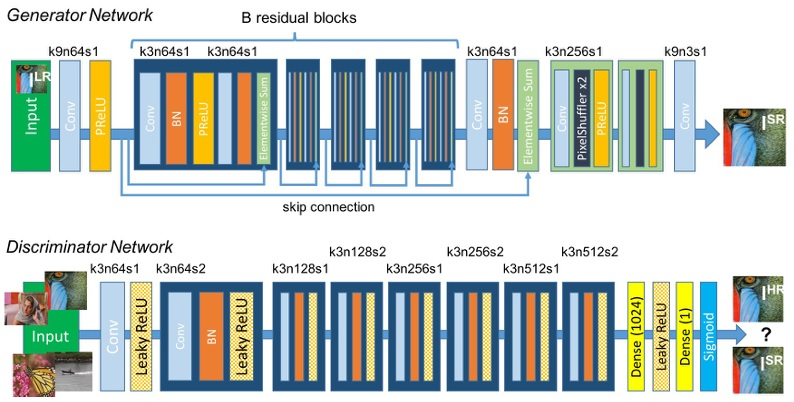
\includegraphics[totalheight=2.5in]{Chapter5/Fig5.1.jpg}
    \caption[Architecture of SRGAN]{Architecture of SRGAN.\cite{SRGAN}}
    \label{fig:label5.1}
\end{figure}

\section{Loss Function of SRGAN}
\subsection{Perceptual loss function}
\begin{equation}
l^{S R}=\underbrace{\underbrace{l_{\mathrm{X}}^{S R}}_{\mathrm{X}}+\underbrace{10^{-3} l_{G e n}^{S R}}_{\text {adversarial loss }}}_{\text {perceptual loss (for VGG based content losses) }}
\end{equation}
\subsection{Content loss function}
The Pixel-wise loss function is given as:
\begin{equation}
l_{M S E}^{S R}=\frac{1}{r^2 W H} \sum_{x=1}^{r W} \sum_{y=1}^{r H}\left(I_{x, y}^{H R}-G_{\theta_G}\left(I^{L R}\right)_{x, y}\right)^2
\end{equation}
This is the most widely used optimization target for image
SR on which many state-of-the-art approaches rely on it. However, while achieving particularly high PSNR, solutions of MSE optimization problems often lack high frequency content which results in perceptually unsatisfying solutions with overly smooth textures.
\subsection{Adversarial loss function}
In addition to the content losses described so far, we also
add the generative component of our GAN to the perceptual
loss. This encourages our network to favor solutions that
reside on the manifold of natural images, by trying to fool the discriminator network. The generative loss ${l_{G e n}^{S R}}$ is defined based on the probabilities of the discriminator ${D_{\theta_D}\left(G_{\theta_G}\left(I^{L R}\right)\right)}$ over all training samples as:
\begin{equation}
l_{G e n}^{S R}=\sum_{n=1}^N-\log D_{\theta_D}\left(G_{\theta_G}\left(I^{L R}\right)\right)
\end{equation}



%\begin{figure}[htb]
%    \centering
%    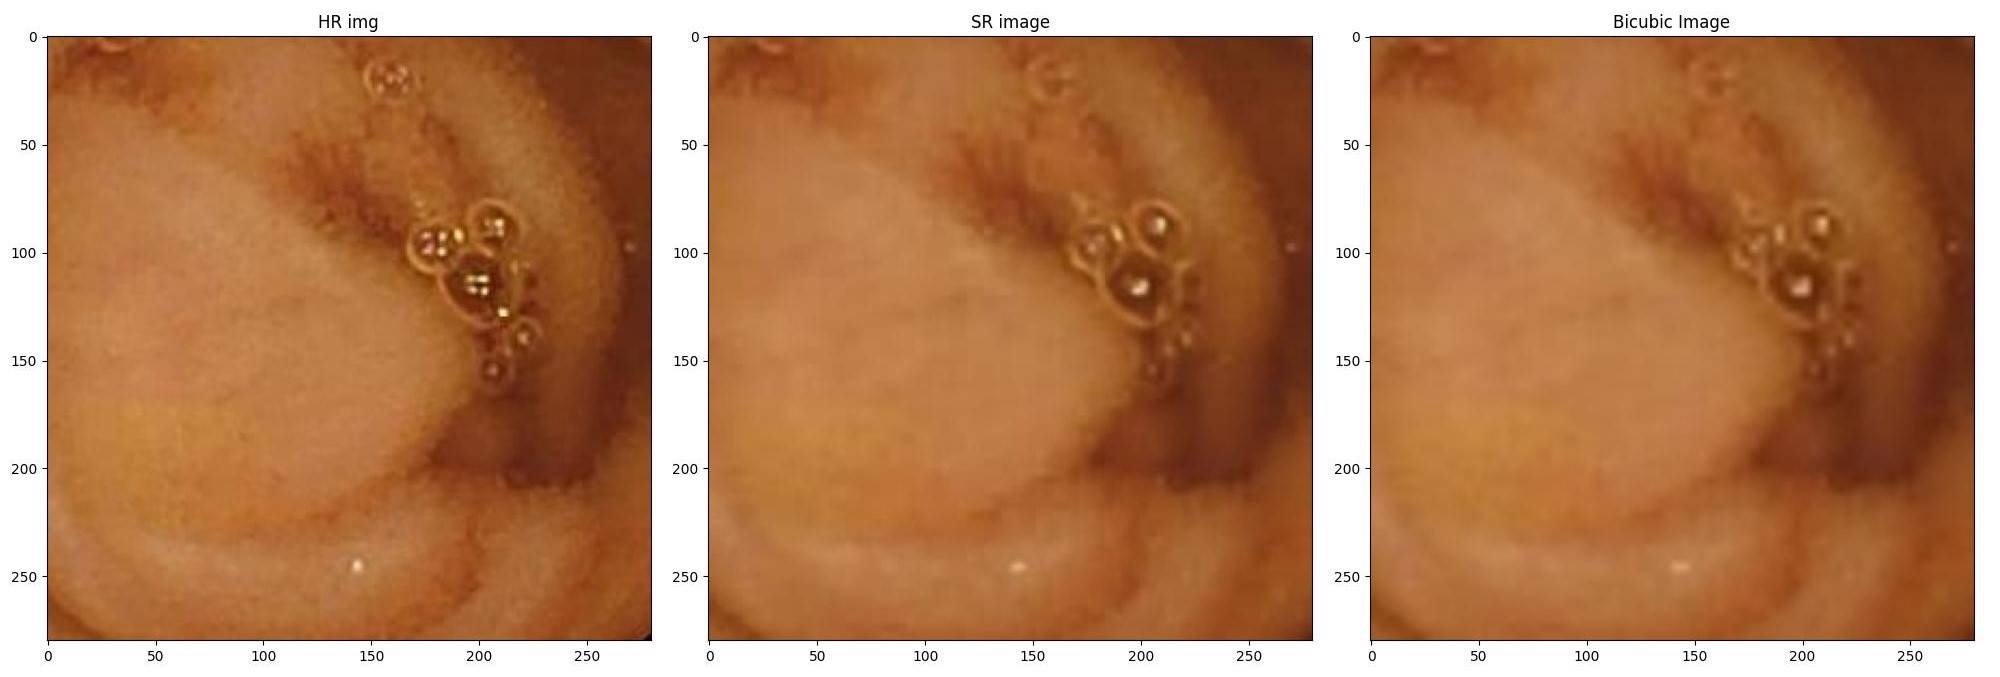
\includegraphics[totalheight=2.0in]{Chapter5/cropped_test (362).jpg}
%    \vspace{0.1}
%    \includegraphics[totalheight=2.0in]{Chapter5/cropped_test %(362)_SSIM.jpg}
%    \caption[SRGAN Generated Image and their SSIM maps]{SRGAN Generated %Image and their SSIM maps.\cite{SRGAN} \cite{SSIM}}
%    \label{fig:label5.4}
%\end{figure}

\section{CycleGAN}
CycleGAN presents an approach for learning to translate an image from a source domain X to a target domain Y in the absence of paired examples. Our goal is to learn a mapping G : X → Y such that the distribution of images from G(X) is indistinguishable from the distribution Y using an adversarial loss. Because this mapping is highly under-constrained, we couple it with an inverse mapping F : Y → X and introduce a cycle consistency loss to enforce F(G(X)) $\thickapprox$ X (and vice versa).


\begin{figure}[h]
    \centering
    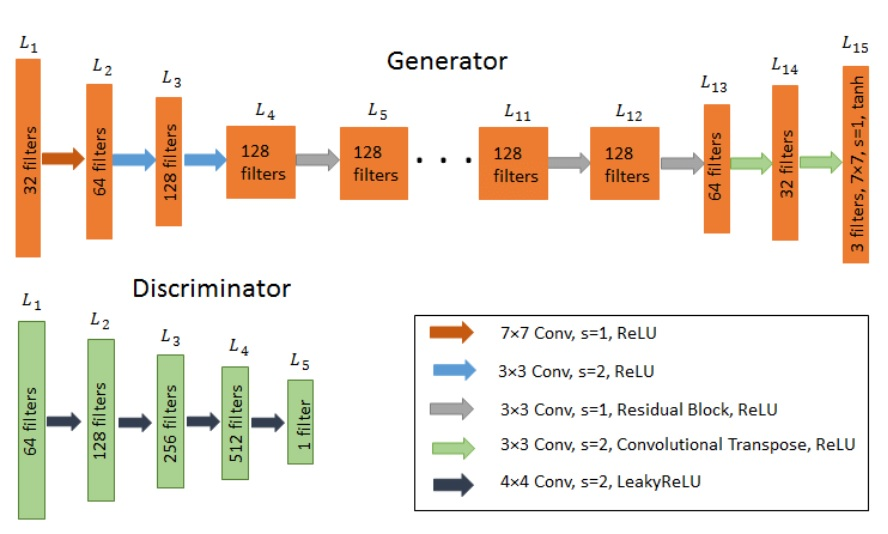
\includegraphics[totalheight=2.5in]{Chapter5/ModelCycle.jpg}
    \caption[Architecture of CycleGAN]{Architecture of CycleGAN.\cite{CycleGAN}}
    \label{fig:label5.8}
\end{figure}

\begin{figure}[h]
    \centering
    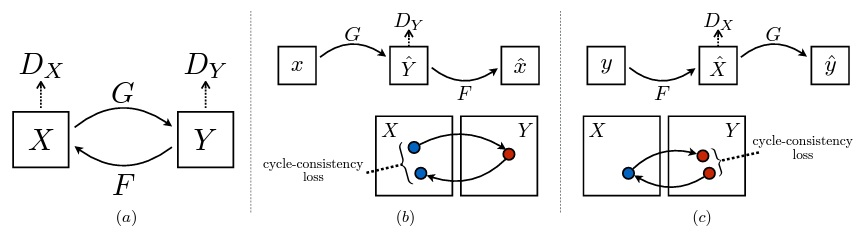
\includegraphics[totalheight=1.5in]{Chapter5/Model.jpg}
    \caption[CycleGAN]{(a) CycleGAN model contains two mapping functions G : X → Y and F : Y → X, and associated adversarial discriminators ${D_Y}$ and ${D_X}$. ${D_Y}$ encourages G to translate X into outputs indistinguishable from domain Y , and vice versa for ${D_X}$ and F. To further regularize the mappings, we introduce two cycle consistency losses that capture the intuition that translates from one domain to the other and back again we should arrive at where we started: (b) forward cycle-consistency loss: {x → G(x) → F(G(x)) $\thickapprox$ x},and (c) backward cycle-consistency loss: y → F(y) → G(F(y))$ \thickapprox $ y .\cite{CycleGAN}}
    \label{fig:label5.5}
\end{figure}

\subsection{Loss in CycleGAN}
\subsubsection{Adversarial Loss}
\begin{equation}
\begin{aligned}
\mathcal{L}_{\mathrm{GAN}}\left(G, D_Y, X, Y\right) &=\mathbb{E}_{y \sim p_{\text {data }}(y)}\left[\log D_Y(y)\right] \\
&+\mathbb{E}_{x \sim p_{\text {data }}(x)}\left[\log \left(1-D_Y(G(x))\right]\right.
\end{aligned}
\end{equation}
where G tries to generate images G(x) that look similar to images from domain Y , while $D_Y$ aims to distinguish between translated samples G(x) and real samples y. G aims to minimize this objective against an adversary D that tries to maximize it, i.e., $min_G$ $max_D_Y$ $L_{GAN}$(G,$D_Y$,X,Y). We introduce a similar adversarial loss for the mapping function F : Y → X and its discriminator $D_X$ as well: i.e., $min_F$ $max_D_X$ $L_{G A N}$(F,$D_X$,Y,X)
\subsubsection{Cycle Consistency Loss}

\begin{equation}
\begin{aligned}
\mathcal{L}_{\text {cyc }}(G, F) &=\mathbb{E}_{x \sim p_{\text {data }}(x)}\left[\|F(G(x))-x\|_1\right] \\
&+\mathbb{E}_{y \sim p_{\text {data }}(y)}\left[\|G(F(y))-y\|_1\right]
\end{aligned}
\end{equation}
\subsubsection{Final Objective}
\begin{equation}
\begin{aligned}
\mathcal{L}\left(G, F, D_X, D_Y\right) &=\mathcal{L}_{\mathrm{GAN}}\left(G, D_Y, X, Y\right) \\
&+\mathcal{L}_{\mathrm{GAN}}\left(F, D_X, Y, X\right) \\
&+\lambda \mathcal{L}_{\text {cyc }}(G, F)
\end{aligned}
\end{equation}


\section{SR Dense-Net}
The proposed network aims to learn an end-to-end mapping function F between the LR image and the HR image. As shown in Fig. \ref{fig:test12}. SRDenseNet can be decomposed into several parts: the convolution layer for learning low-level feature, the blocks of DenseNet for learning highlevel features, the deconvolution layers for learning upscaling filters and the reconstruction layer for generating the HR output. Each convolution or deconvolution layer is followed by a ReLu layer for nonlinear mapping except the reconstruction layer. The ReLu activation function is applied element-wise. 
 \begin{figure}[H]
    \centering
    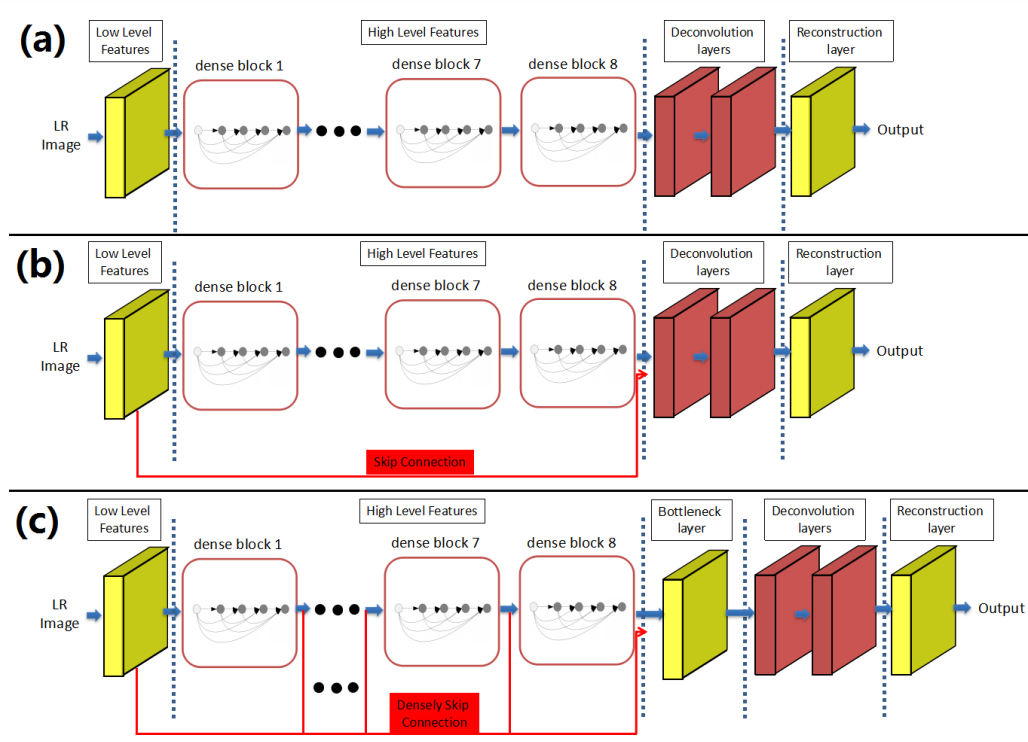
\includegraphics[totalheight=2.8in]{Chapter5/image21.png}
    \caption{Architectures of different SR-Dense Models}
    \label{fig:test12}
\end{figure}

Different structures of the proposed networks.\\
 (a) SRDenseNet H: only the high-level feature maps are used as input for reconstructing the HR images. \\
(b) SRDenseNet HL: the low-level and the high-level features are combined as input for reconstructing the HR images. \\
(c) SRDenseNet All: all levels of features are combined via skip connections as input for reconstructing the HR images. \\
We minimize the following Mean Squared Error (MSE). Adam is used to find the optimum weights and biases in the above equation. In the following, we will describe the details of the proposed network structures.

\subsection{SR Dense-Net blocks}
After applying a convolution layer to the input LR images for learning low-level features, a set of DenseNet blocks are adopted for learning the high-level features.

 In the structure of DenseNet, short paths are created between a layer and every other layer. This strengthens the flow of information through deep networks, thus alleviating the vanishing-gradient problem. In addition, DenseNet can substantially reduce the number of parameters through feature reuse, thus requiring less memory and computation to achieve high performance [7]. Here, we employ the DenseNet structure as a building block in our network. The structure of each denseNet block can be seen in Fig. \ref{fig:test13} Specifically, there are 8 convolution layers in one DenseNet block in our work. If each convolution layer produce k feature maps as output, the total number of feature maps generated by one DenseNet block is k ∗ 8, where k is refered to as growth rate. The growth rate k regulates how much new information each layer contributes to the final reconstruction. To prevent the network from growing too wide, the growth rate k is set to 16 in this study. This results in a total number of 128 feature maps from one DenseNet block. 

\begin{figure}[H]
    \centering
    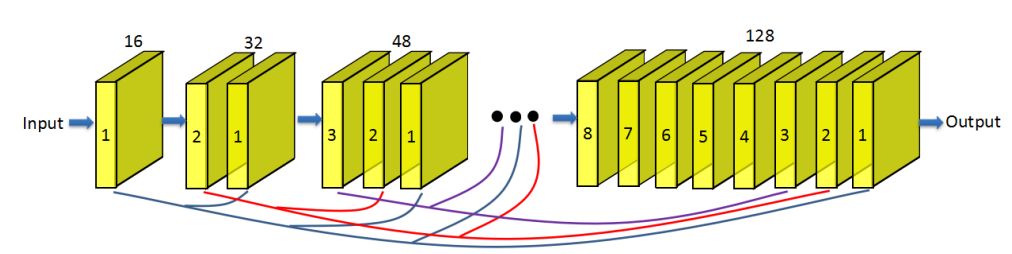
\includegraphics[totalheight=1.4in]{Chapter5/image22.png}
    \caption{The structure of one DenseNet block.}
    \label{fig:test13}
\end{figure}



\section{RCAN}

Most recent CNN-based methods treat channel-wise features equally, which lacks flexibility in dealing with different types of information. Image SR can be viewed as a process, where we try to recover as more high-frequency information as possible. The LR images contain most low-frequency information, which can directly forwarded to the final HR outputs. While, the leading CNN-based methods would treat each channel-wise feature equally, lacking discriminative learning ability across feature channels, and hindering the representational power of deep networks.  

\begin{figure}[H]
    \centering
    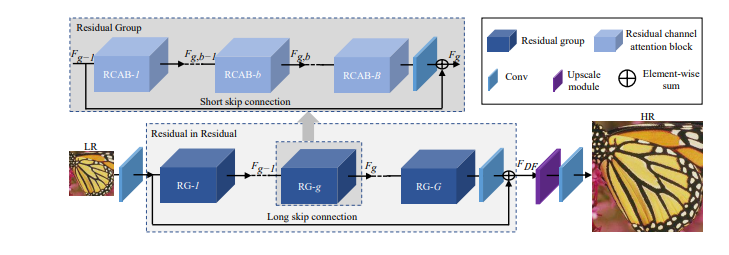
\includegraphics[totalheight=2.0in]{Chapter5/image23.png}
    \caption{Network Architecture of RCAN}
    \label{fig:test14}
\end{figure}

After conducting series on experiments on state of art models, we came to an conclusion that the modalities of capsule endsocopy dataset are very well learned and captured by networks with dense connections.
